\documentclass[12pt,chapterheads,oneside]{ucsd}

\usepackage{amsmath, amscd, amssymb, amsthm}
\usepackage{graphicx}
\usepackage{xfrac}
\usepackage{color}
\usepackage{multirow}
\usepackage{multicol}
\usepackage{ifthen}
\usepackage{xspace}
\usepackage{calc}
\usepackage{diagbox}
\usepackage{subfig}
\usepackage[T1]{fontenc}
\usepackage{mathptmx}
\usepackage{makeidx}
\usepackage[bottom]{footmisc}
\usepackage[hyphens]{url}
\usepackage[color=red!40,textwidth=24mm,textsize=footnotesize]{todonotes}
\usepackage[hidelinks,linktocpage,breaklinks]{hyperref}                                  
\usepackage{rotating}
\usepackage{afterpage}
\usepackage{xparse}
\usepackage{lineno}
\usepackage{slashed}
\usepackage{bm}
\usepackage{ragged2e}
\usepackage{lmodern}% http://ctan.org/pkg/lm
%% \usepackage[style=base]{caption}
%% \captionsetup{style=base}
\usepackage{url}

\hypersetup{ pdfauthor   = {Doe, John},
             pdftitle    = {The Title},
             pdfkeywords = {},
             pdfcreator  = {LaTeX with hyperref package},
             pdfproducer = {LaTeX} }

%%%%%%%%%%%%%%%%%%%%%%%%%%%%%%%%%%%%%%%%%%%%%%%%%%%%%%%%%%%%%%%%%%%%
%
%  CMS Common definitions style file
%
%  N.B. use of \newcommand rather than \newcommand means
%       that a definition is ignored if already specified
%
%                                              L. Taylor 18 Feb 2005
%%%%%%%%%%%%%%%%%%%%%%%%%%%%%%%%%%%%%%%%%%%%%%%%%%%%%%%%%%%%%%%%%%%%

% Some shorthand
% turn off italics
\newcommand {\etal}{\mbox{et al.}\xspace} %et al. - no preceding comma
\newcommand {\ie}{\mbox{i.e.}\xspace}     %i.e.
\newcommand {\eg}{\mbox{e.g.}\xspace}     %e.g.
\newcommand {\etc}{\mbox{etc.}\xspace}     %etc.
\newcommand {\vs}{\mbox{\sl vs.}\xspace}      %vs.
\newcommand {\mdash}{\ensuremath{\mathrm{-}}} % for use within formulas

% some terms whose definition we may change
\newcommand {\Lone}{Level-1\xspace} % Level-1 or L1 ?
\newcommand {\Ltwo}{Level-2\xspace}
\newcommand {\Lthree}{Level-3\xspace}

% Some software programs (alphabetized)
\newcommand{\ACERMC} {\textsc{AcerMC}\xspace}
\newcommand{\ALPGEN} {{\textsc{alpgen}}\xspace}
\newcommand{\CHARYBDIS} {{\textsc{charybdis}}\xspace}
\newcommand{\CMKIN} {\textsc{cmkin}\xspace}
\newcommand{\CMSIM} {{\textsc{cmsim}}\xspace}
\newcommand{\CMSSW} {{\textsc{cmssw}}\xspace}
\newcommand{\COBRA} {{\textsc{cobra}}\xspace}
\newcommand{\COCOA} {{\textsc{cocoa}}\xspace}
\newcommand{\COMPHEP} {\textsc{CompHEP}\xspace}
\newcommand{\CTTEN} {\textsc{cteq10}\xspace}
\newcommand{\EVTGEN} {{\textsc{evtgen}}\xspace}
\newcommand{\FAMOS} {{\textsc{famos}}\xspace}
\newcommand{\GARCON} {\textsc{garcon}\xspace}
\newcommand{\GARFIELD} {{\textsc{garfield}}\xspace}
\newcommand{\GEANE} {{\textsc{geane}}\xspace}
\newcommand{\GEANTfour} {{\textsc{geant4}}\xspace}
\newcommand{\GEANTthree} {{\textsc{geant3}}\xspace}
\newcommand{\GEANT} {{\textsc{geant}}\xspace}
\newcommand{\HDECAY} {\textsc{hdecay}\xspace}
\newcommand{\HERWIG} {{\textsc{herwig}}\xspace}
\newcommand{\HIGLU} {{\textsc{higlu}}\xspace}
\newcommand{\HIJING} {{\textsc{hijing}}\xspace}
\newcommand{\IGUANA} {\textsc{iguana}\xspace}
\newcommand{\ISAJET} {{\textsc{isajet}}\xspace}
\newcommand{\ISAPYTHIA} {{\textsc{isapythia}}\xspace}
\newcommand{\ISASUGRA} {{\textsc{isasugra}}\xspace}
\newcommand{\ISASUSY} {{\textsc{isasusy}}\xspace}
\newcommand{\ISAWIG} {{\textsc{isawig}}\xspace}
\newcommand{\JIMMY} {{\textsc{jimmy}}\xspace}
\newcommand{\MADGRAPH} {\textsc{MadGraph}\xspace}
\newcommand{\MSTW} {\textsc{mstw2008}\xspace}
\newcommand{\NNPDF} {\textsc{nnpdf}\xspace}
\newcommand{\GGTWW}  {{\textsc{gg2ww}}\xspace}
\newcommand{\POWHEG} {\textsc{powheg}\xspace}
\newcommand{\HqT} {\textsc{HqT}\xspace}
\newcommand{\MCATNLO} {\textsc{mc@nlo}\xspace}
\newcommand{\MCFM} {\textsc{mcfm}\xspace}
\newcommand{\FEWZ} {\textsc{fewz}\xspace}
\newcommand{\MILLEPEDE} {{\textsc{millepede}}\xspace}
\newcommand{\ORCA} {{\textsc{orca}}\xspace}
\newcommand{\OSCAR} {{\textsc{oscar}}\xspace}
\newcommand{\PHOTOS} {\textsc{photos}\xspace}
\newcommand{\PROSPINO} {\textsc{prospino}\xspace}
\newcommand{\PYTHIA} {{\textsc{pythia}}\xspace}
\newcommand{\SHERPA} {{\textsc{sherpa}}\xspace}
\newcommand{\TAUOLA} {\textsc{tauola}\xspace}
\newcommand{\TOPREX} {\textsc{TopReX}\xspace}
\newcommand{\XDAQ} {{\textsc{xdaq}}\xspace}


%  Experiments
\newcommand {\DZERO}{D0\xspace}     %etc.


% Measurements and units...

\newcommand{\de}{\ensuremath{^\circ}}
\newcommand{\ten}[1]{\ensuremath{\times \text{10}^\text{#1}}}
\newcommand{\unit}[1]{\ensuremath{\text{\,#1}}\xspace}
\newcommand{\mum}{\ensuremath{\,\mu\text{m}}\xspace}
\newcommand{\micron}{\ensuremath{\,\mu\text{m}}\xspace}
\newcommand{\cm}{\ensuremath{\,\text{cm}}\xspace}
\newcommand{\cmcm}{\ensuremath{\,\text{cm^2}}\xspace}
\newcommand{\s}{\ensuremath{\,\text{s}}\xspace}
\newcommand{\ns}{\ensuremath{\,\text{ns}}\xspace}
% \newcommand{\mm}{\ensuremath{\,\text{mm}}\xspace}
\newcommand{\mus}{\ensuremath{\,\mu\text{s}}\xspace}
\newcommand{\keV}{\ensuremath{\,\text{ke\hspace{-.08em}V}}\xspace}
\newcommand{\MeV}{\ensuremath{\,\text{Me\hspace{-.08em}V}}\xspace}
\newcommand{\GeV}{\ensuremath{\,\text{Ge\hspace{-.08em}V}}\xspace}
\newcommand{\gev}{\GeV}
\newcommand{\TeV}{\ensuremath{\,\text{Te\hspace{-.08em}V}}\xspace}
\newcommand{\PeV}{\ensuremath{\,\text{Pe\hspace{-.08em}V}}\xspace}
\newcommand{\keVc}{\ensuremath{{\,\text{ke\hspace{-.08em}V\hspace{-0.16em}/\hspace{-0.08em}}c}}\xspace}
\newcommand{\MeVc}{\ensuremath{{\,\text{Me\hspace{-.08em}V\hspace{-0.16em}/\hspace{-0.08em}}c}}\xspace}
\newcommand{\GeVc}{\ensuremath{{\,\text{Ge\hspace{-.08em}V\hspace{-0.16em}/\hspace{-0.08em}}c}}\xspace}
\newcommand{\TeVc}{\ensuremath{{\,\text{Te\hspace{-.08em}V\hspace{-0.16em}/\hspace{-0.08em}}c}}\xspace}
\newcommand{\keVcc}{\ensuremath{{\,\text{ke\hspace{-.08em}V\hspace{-0.16em}/\hspace{-0.08em}}c^\text{2}}}\xspace}
\newcommand{\MeVcc}{\ensuremath{{\,\text{Me\hspace{-.08em}V\hspace{-0.16em}/\hspace{-0.08em}}c^\text{2}}}\xspace}
\newcommand{\GeVcc}{\ensuremath{{\,\text{Ge\hspace{-.08em}V\hspace{-0.16em}/\hspace{-0.08em}}c^\text{2}}}\xspace}
\newcommand{\TeVcc}{\ensuremath{{\,\text{Te\hspace{-.08em}V\hspace{-0.16em}/\hspace{-0.08em}}c^\text{2}}}\xspace}

\newcommand{\barn} {\mbox{\ensuremath{\,\text{b}}}\xspace}
\newcommand{\binv} {\mbox{\ensuremath{\,\text{b}^\text{$-$1}}}\xspace}
\newcommand{\pb} {\mbox{\ensuremath{\,\text{pb}}}\xspace}
\newcommand{\fb} {\mbox{\ensuremath{\,\text{fb}}}\xspace}
\newcommand{\pbinv} {\mbox{\ensuremath{\,\text{pb}^\text{$-$1}}}\xspace}
\newcommand{\fbinv} {\mbox{\ensuremath{\,\text{fb}^\text{$-$1}}}\xspace}
\newcommand{\usedLumi} {\mbox{\ensuremath{19.5\,\text{fb}^\text{$-$1}}}\xspace}
\newcommand{\nbinv} {\mbox{\ensuremath{\,\text{nb}^\text{$-$1}}}\xspace}
\newcommand{\percms}{\ensuremath{\,\text{cm}^\text{$-$2}\,\text{s}^\text{$-$1}}\xspace}
\newcommand{\lumi}{\ensuremath{\mathcal{L}}\xspace}
\newcommand{\Lumi}{\ensuremath{\mathcal{L}}\xspace}%both upper and lower
%
% Need a convention here:
\newcommand{\LvLow}  {\ensuremath{\mathcal{L}=\text{10}^\text{32}\,\text{cm}^\text{$-$2}\,\text{s}^\text{$-$1}}\xspace}
\newcommand{\LLow}   {\ensuremath{\mathcal{L}=\text{10}^\text{33}\,\text{cm}^\text{$-$2}\,\text{s}^\text{$-$1}}\xspace}
\newcommand{\lowlumi}{\ensuremath{\mathcal{L}=\text{2}\times \text{10}^\text{33}\,\text{cm}^\text{$-$2}\,\text{s}^\text{$-$1}}\xspace}
\newcommand{\LMed}   {\ensuremath{\mathcal{L}=\text{2}\times \text{10}^\text{33}\,\text{cm}^\text{$-$2}\,\text{s}^\text{$-$1}}\xspace}
\newcommand{\LHigh}  {\ensuremath{\mathcal{L}=\text{10}^\text{34}\,\text{cm}^\text{$-$2}\,\text{s}^\text{$-$1}}\xspace}
\newcommand{\hilumi} {\ensuremath{\mathcal{L}=\text{10}^\text{34}\,\text{cm}^\text{$-$2}\,\text{s}^\text{$-$1}}\xspace}

% Physics symbols ...

\newcommand{\dzero}{\ensuremath{d_{\mathrm{0}}}\xspace}
\newcommand{\dz}{\ensuremath{d_{\mathrm{z}}}\xspace}
\newcommand{\PT}{\ensuremath{p_{\mathrm{T}}}\xspace}
\newcommand{\pt}{\ensuremath{p_{\mathrm{T}}}\xspace}
\newcommand{\ET}{\ensuremath{E_{\mathrm{T}}}\xspace}
\newcommand{\HT}{\ensuremath{H_{\mathrm{T}}}\xspace}
\newcommand{\vHT}{\ensuremath{\vec{H}_{\mathrm{T}}}\xspace}
\newcommand{\et}{\ensuremath{E_{\mathrm{T}}}\xspace}
\newcommand{\Em}{\ensuremath{E\hspace{-0.6em}/}\xspace}
\newcommand{\Pm}{\ensuremath{p\hspace{-0.5em}/}\xspace}
\newcommand{\PTm}{\ensuremath{{p}_\mathrm{T}\hspace{-1.02em}/}\xspace}
\newcommand{\PTslash}{\ensuremath{{p}_\mathrm{T}\hspace{-1.02em}/}\xspace}
\newcommand{\ETm}{\ensuremath{E_{\mathrm{T}}^{\text{miss}}}\xspace}
\newcommand{\vMET}{\ensuremath{\vec{E}_{\mathrm{T}}^{\text{miss}}}\xspace}
\newcommand{\MET}{\ETm}
\newcommand{\ETmiss}{\ETm}
\newcommand{\ETslash}{\ensuremath{E_{\mathrm{T}}\hspace{-1.1em}/\kern0.45em}\xspace}
\newcommand{\VEtmiss}{\ensuremath{{\vec E}_{\mathrm{T}}^{\text{miss}}}\xspace}

% roman face derivative
\newcommand{\dd}[2]{\ensuremath{\frac{\mathrm{d} #1}{\mathrm{d} #2}}}
\newcommand{\ddinline}[2]{\ensuremath{\mathrm{d} #1/\mathrm{d} #2}}
% absolute value
\newcommand{\abs}[1]{\ensuremath{\lvert #1 \rvert}}

% SS definintions
\newcommand{\hpt}{high \ensuremath{p_{T}}\xspace}
\newcommand{\lpt}{low \ensuremath{p_{T}}\xspace}
\newcommand{\vpt}{very low \ensuremath{p_{T}}\xspace}


% \ifthenelse{\boolean{cms@italic}}{\newcommand{\cmsSymbolFace}{\relax}}{\newcommand{\cmsSymbolFace}{\mathrm}}
\newcommand{\cmsSymbolFace}{\relax}                                            
% \newcommand{\cmsSymbolFace}{\mathrm}                                           

% I think this came from the OS definitions
\newcommand{\z}{$Z$ }
\newcommand{\zjets}{$\rm{Z}+\rm{jets}$ }
\newcommand{\zbb}{$\rm{Z+b\bar{b}}$ }
\newcommand{\gjets}{$\gamma+\rm{jets}$ }
\newcommand{\ttV}{\ensuremath{t\bar{t}\rm{V}}}
%% \newcommand{\emu}{\ensuremath{e\mu}}
\newcommand{\eepm}{\ensuremath{e^+ e^-}}
\newcommand{\mmpm}{\ensuremath{\mu^+ \mu^-}}
\newcommand{\empm}{\ensuremath{e^\pm \mu^\mp}}
\newcommand{\ase}[2]{\ensuremath{_{~- #1}^{~+ #2}}}
\newcommand{\effr}{$R_{e\mu}$} %used to be \epsilon
\newcommand{\effrm}{$R_{\mu e}$} %used to be \epsilon
\newcommand{\sta}{$\sigma\times A$} %notation is such that A includes BR
\newcommand{\statistics}{CL$_\mathrm{S}$}
\newcommand{\MTj}{\ensuremath{\rm{M_{T2}^{j}}}}
\newcommand{\MT}{\ensuremath{\rm{M_{T2}}}}
\newcommand{\mbb}{\ensuremath{\rm{M_{\bbbar}}}}
\newcommand{\chizi}{\ensuremath{\tilde{\chi}^{0}_{1}}}
\newcommand{\chizii}{\ensuremath{\tilde{\chi}^{0}_{2}}}
\newcommand{\wjets}{$\rm{W}+{\rm jets}$}
\newcommand{\zzmet}{$\rm{ZZ}+\MET$}
\newcommand{\wzmet}{$\rm{WZ}+\MET$}
\newcommand{\wzzmet}{$\rm{WZ/ZZ}+\MET$}
\newcommand{\cls}  {\ensuremath{\mathrm{CL_S}}}


% Extensions for missing names in PENNAMES % note no xspace, to match syntax in PENNAMES
\newcommand{\Paq}{\ensuremath{\cmsSymbolFace{\overline{q}}}}
\newcommand{\Pq}{\ensuremath{\cmsSymbolFace{q}}}
\newcommand{\PWm}{\ensuremath{{\cmsSymbolFace{W^-}}}}
\newcommand{\PWp}{\ensuremath{{\cmsSymbolFace{W^+}}}}
\newcommand{\Pp}{\ensuremath{\cmsSymbolFace{p}}}
\newcommand{\cPgn}{\ensuremath{\nu}} % generic neutrino
\newcommand{\cPagn}{\ensuremath{\overline{\nu}}} % generic neutrino
\newcommand{\cPgg}{\ensuremath{\gamma}} % gamma
\newcommand{\cPJgy}{\ensuremath{\cmsSymbolFace{J}\hspace{-.08em}/\hspace{-.14em}\psi}} % J/Psi (no mass)
\newcommand{\cPZ}{\ensuremath{\cmsSymbolFace{Z}}} % plain Z (no superscript 0)
\newcommand{\cPZpr}{\ensuremath{\cmsSymbolFace{Z}^\prime}} % plain Z'
\newcommand{\cPqt}{\ensuremath{\cmsSymbolFace{t}}} % t for t quark
\newcommand{\cPqb}{\ensuremath{\cmsSymbolFace{b}}} % b for b quark
\newcommand{\cPqc}{\ensuremath{\cmsSymbolFace{c}}} % c for c quark
\newcommand{\cPqs}{\ensuremath{\cmsSymbolFace{s}}} % s for s quark
\newcommand{\cPqu}{\ensuremath{\cmsSymbolFace{u}}} % u for u quark
\newcommand{\cPqd}{\ensuremath{\cmsSymbolFace{d}}} % d for d quark
\newcommand{\cPq}{\ensuremath{\cmsSymbolFace{q}}} % generic quark
\newcommand{\cPg}{\ensuremath{\cmsSymbolFace{g}}} % generic gluon
\newcommand{\cPG}{\ensuremath{\cmsSymbolFace{G}}} % Graviton
\newcommand{\cPaqt}{\ensuremath{\overline{\cmsSymbolFace{t}}}} % t for t anti-quark
\newcommand{\cPaqb}{\ensuremath{\overline{\cmsSymbolFace{b}}}} % b for b anti-quark
\newcommand{\cPaqc}{\ensuremath{\overline{\cmsSymbolFace{c}}}} % c for c anti-quark
\newcommand{\cPaqs}{\ensuremath{\overline{\cmsSymbolFace{s}}}} % s for s anti-quark
\newcommand{\cPaqu}{\ensuremath{\overline{\cmsSymbolFace{u}}}} % u for u anti-quark
\newcommand{\cPaqd}{\ensuremath{\overline{\cmsSymbolFace{d}}}} % d for d anti-quark
\newcommand{\cPaq}{\ensuremath{\overline{\cmsSymbolFace{q}}}} % generic anti-quark
% future symbols from heppennames
% \providecommand{\PH}{\ensuremath{\cmsSymbolFace{H}}\xspace} % plain Higgs
% \providecommand{\PJGy}{\ensuremath{\cmsSymbolFace{J}\hspace{-.08em}/\hspace{-.14em}\psi}\xspace} % J/Psi (no mass)
% \providecommand{\PBzs}{\ensuremath{\cmsSymbolFace{B}^0_\cmsSymbolFace{s}}\xspace} % B^0_s
\newcommand{\relIso}{\ensuremath{Iso}\xspace}

% Particle names which track the italic/non-italic face convention
\newcommand{\zp}{\ensuremath{\cmsSymbolFace{Z}^\prime}\xspace} % plain Z'
\newcommand{\JPsi}{\ensuremath{\cmsSymbolFace{J}\hspace{-.08em}/\hspace{-.14em}\psi}\xspace} % J/Psi (no mass)
\newcommand{\Z}{\ensuremath{\cmsSymbolFace{Z}}\xspace} % plain Z (no superscript 0)
\newcommand{\epem}{\ensuremath{\cmsSymbolFace{e^{+}e^{-}}}\xspace} % e+e- 
\newcommand{\tW}{\ensuremath{\cmsSymbolFace{t}\cmsSymbolFace{W}}\xspace} % t-tbar
\newcommand{\PH}{\ensuremath{\cmsSymbolFace{H}}\xspace} % plain Higgs
\newcommand{\Pe}{\ensuremath{\cmsSymbolFace{e}}\xspace} % plain Higgs
\newcommand{\WW}{\ensuremath{\cmsSymbolFace{WW}}\xspace} 
\newcommand{\WpWm}{\ensuremath{\W^+\W^-}\xspace} 
\newcommand{\HWW}{\ensuremath{\PH\to\WpWm}\xspace} 
\newcommand{\HWWllnn}{\ensuremath{\PH\to\WpWm\to\ell\nu\ell^\prime\overline{\nu}}\xspace} 
\newcommand{\Wgamma}{\ensuremath{\cmsSymbolFace{W}\gamma}\xspace} 
\newcommand{\HZZ}{\ensuremath{\PH\to\ZZ}\xspace} 
\newcommand{\Hgg}{\ensuremath{\PH\to\gamma\gamma}\xspace} 
\newcommand{\ggWW}{\ensuremath{\cmsSymbolFace{gg}\to\cmsSymbolFace{WW}}\xspace} 
\newcommand{\ggH}{\ensuremath{\cmsSymbolFace{gg}\to\cmsSymbolFace{H}}\xspace} 

\newcommand{\ee}{\ensuremath{\cmsSymbolFace{ee}}\xspace} 
\newcommand{\mm}{\ensuremath{\cmsSymbolFace{\mu\mu}}\xspace} 
%% \renewcommand{\em}{\ensuremath{\cmsSymbolFace{e\mu}}\xspace} 
\newcommand{\me}{\ensuremath{\cmsSymbolFace{\mu e}}\xspace} 
\renewcommand{\ll}{\ensuremath{\cmsSymbolFace{\ell\ell}}\xspace} 
\newcommand{\bj}{\ensuremath{\cmsSymbolFace{b}}-tagged jet\xspace} 
\newcommand{\bjs}{\ensuremath{\cmsSymbolFace{b}}-tagged jets\xspace} 
\newcommand{\bqs}{\ensuremath{\cmsSymbolFace{b}}-quarks\xspace} 
\newcommand{\bq}{\ensuremath{\cmsSymbolFace{b}}-quark\xspace} 
\newcommand{\njets}{\ensuremath{\mathrm{N_{jets}}}} 
\newcommand{\nbtags}{\ensuremath{\mathrm{N_{b-tags}}}} 
\newcommand{\btag}{\ensuremath{\cmsSymbolFace{b}}-tag\xspace} 
\newcommand{\btagged}{\ensuremath{\cmsSymbolFace{b}}-tagged\xspace} 
\newcommand{\tnp}{tag-and-probe\xspace} 
\newcommand{\dmc}{data-to-simulation\xspace} 

\newcommand{\ttbar}{\ensuremath{\cmsSymbolFace{t}\overline{\cmsSymbolFace{t}}}\xspace} % t-tbar
\newcommand{\ttdil}{\ensuremath{\ttbar\to\ell\ell X}}               % t-tbar --> 2 x lnb
\newcommand{\ttslb}{\ensuremath{\ttbar\to\ell(b\to\ell) X}}         % t-tbar --> lnb + jjb
\newcommand{\ttslo}{\ensuremath{\ttbar\to\ell(b\!\!\!/\to\ell) X}}  % t-tbar --> not lnb + jjb 
\newcommand{\ttslq}{\ensuremath{\ttbar\to\ell(q\to\ell) X}}         % t-tbar --> lnb + jjb
\newcommand{\tthad}{\ensuremath{\ttbar\to\rm{hadronic}}}            % t-tbar --> hadronic
\newcommand{\ttZ}{\ensuremath{\cmsSymbolFace{t}\overline{\cmsSymbolFace{t}}\cmsSymbolFace{Z}}\xspace} % t-tbar Z
\newcommand{\ttW}{\ensuremath{\cmsSymbolFace{t}\overline{\cmsSymbolFace{t}}\cmsSymbolFace{W}}\xspace} % t-tbar W
\newcommand{\ttWW}{\ensuremath{\cmsSymbolFace{t}\overline{\cmsSymbolFace{t}}\cmsSymbolFace{W}\cmsSymbolFace{W}}\xspace} % t-tbar WW
\newcommand{\ttG}{\ensuremath{\cmsSymbolFace{t}\overline{\cmsSymbolFace{t}}\cmsSymbolFace{\gamma}}\xspace} % t-tbar G
\newcommand{\tbZ}{\ensuremath{\cmsSymbolFace{t}\overline{\cmsSymbolFace{b}}\cmsSymbolFace{Z}}\xspace} % t-bbar Z
\newcommand{\WWG}{\ensuremath{\cmsSymbolFace{WW\gamma}}\xspace} 
\newcommand{\WWW}{\ensuremath{\cmsSymbolFace{WWW}}\xspace} 
\newcommand{\WWZ}{\ensuremath{\cmsSymbolFace{WWZ}}\xspace} 
\newcommand{\WZZ}{\ensuremath{\cmsSymbolFace{WZZ}}\xspace} 
\newcommand{\ZZZ}{\ensuremath{\cmsSymbolFace{ZZZ}}\xspace} 
\newcommand{\WZ}{\ensuremath{\cmsSymbolFace{WZ}}\xspace} 
\newcommand{\ZZ}{\ensuremath{\cmsSymbolFace{ZZ}}\xspace} 
\newcommand{\qqWW}{\ensuremath{\cmsSymbolFace{qqW^{\pm}W^{\pm}}}\xspace} 
\newcommand{\qqWmWm}{\ensuremath{\cmsSymbolFace{qqW^{-}W^{-}}}\xspace} 
\newcommand{\qqWpWp}{\ensuremath{\cmsSymbolFace{qqW^{+}W^{+}}}\xspace} 
\newcommand{\WWdps}{\ensuremath{\cmsSymbolFace{W^{\pm}W^{\pm}}(DPS)}\xspace} 
\newcommand{\Wgs}{\ensuremath{\cmsSymbolFace{W}\gamma^{*}}\xspace} 
\newcommand{\Wgsmm}{\ensuremath{\cmsSymbolFace{W}\gamma^{*} \to \ell\nu\mu\mu}\xspace} 
\newcommand{\Wgsee}{\ensuremath{\cmsSymbolFace{W}\gamma^{*} \to \ell\nuee}\xspace} 
\newcommand{\Wgstt}{\ensuremath{\cmsSymbolFace{W}\gamma^{*} \to \ell\nu\tau\tau}\xspace} 
\newcommand{\HToZZ}{\ensuremath{WH, ZH, \ttbar H;\ H\to\ZZ}\xspace} 
\newcommand{\HToWW}{\ensuremath{WH, ZH, \ttbar H;\ H\to\WW}\xspace} 
\newcommand{\HToTauTau}{\ensuremath{WH, ZH, \ttbar H;\ H\to\tau\tau}\xspace} 

% SM (still to be classified)

\newcommand{\AFB}{\ensuremath{A_\text{FB}}\xspace}
\newcommand{\wangle}{\ensuremath{\sin^{2}\theta_{\text{eff}}^\text{lept}(M^2_\Z)}\xspace}
\newcommand{\stat}{\ensuremath{\,\text{(stat.)}}\xspace}
\newcommand{\syst}{\ensuremath{\,\text{(syst.)}}\xspace}
\newcommand{\kt}{\ensuremath{k_{\mathrm{T}}}\xspace}

\newcommand{\BC}{\ensuremath{\cmsSymbolFace{B_{c}}}\xspace}
\newcommand{\bbarc}{\ensuremath{\cPqb\cPaqc}\xspace}
\newcommand{\bbbar}{\ensuremath{\cPqb\cPaqb}\xspace}
\newcommand{\ccbar}{\ensuremath{\cPqc\cPaqc}\xspace}
\newcommand{\bspsiphi}{\ensuremath{\cmsSymbolFace{B_s} \to \JPsi\, \phi}\xspace}
\newcommand{\EE}{\ensuremath{\Pep\Pem}\xspace}
\newcommand{\MM}{\ensuremath{\Pgmp\Pgmm}\xspace}
\newcommand{\TT}{\ensuremath{\Pgt^{+}\Pgt^{-}}\xspace}

%%%  E-gamma definitions
% \newcommand{\HGG}{\ensuremath{\cmsSymbolFace{H}\to\gamma\gamma}\xspace}        
% \newcommand{\GAMJET}{\ensuremath{\gamma + \text{jet}}\xspace}                  
\newcommand{\gs}{\ensuremath{\gamma^{*}}\xspace}
\newcommand{\gj}{\ensuremath{\gamma + \text{jets}}\xspace}
\newcommand{\Wj}{\ensuremath{\W + \text{jets}}\xspace}
\newcommand{\Zj}{\ensuremath{\Z + \text{jets}}\xspace}
\newcommand{\Wlnu}{\ensuremath{\W \to \ell\bar{\nu}_{\ell}}\xspace}
\newcommand{\Wplpnu}{\ensuremath{\W^+ \to \ell^+\bar{\nu}_{\ell}}\xspace}
\newcommand{\Wmlmnu}{\ensuremath{\W^- \to \ell^-\bar{\nu}_{\ell}}\xspace}
\newcommand{\Wpmlpmnu}{\ensuremath{\W^{\pm} \to \ell^{\pm}\bar{\nu}_{\ell}}\xspace}
\newcommand{\Wqq}{\ensuremath{\W \to q\bar{q}}\xspace}
% \newcommand{\PPTOJETS}{\ensuremath{\Pp\Pp\to\text{jets}}\xspace}               
% \newcommand{\PPTOGG}{\ensuremath{\Pp\Pp\to\gamma\gamma}\xspace}                
% \newcommand{\PPTOGAMJET}{\ensuremath{\Pp\Pp\to\gamma + \mathrm{jet}}\xspace}   
% \newcommand{\MH}{\ensuremath{M_{\mathrm{H}}}\xspace}                           
% \newcommand{\RNINE}{\ensuremath{R_\mathrm{9}}\xspace}                          





%%%%%%
% From Albert
%

\newcommand{\ga}{\ensuremath{\gtrsim}}
\newcommand{\la}{\ensuremath{\lesssim}}
%
\newcommand{\swsq}{\ensuremath{\sin^2\theta_\cmsSymbolFace{W}}\xspace}
\newcommand{\cwsq}{\ensuremath{\cos^2\theta_\cmsSymbolFace{W}}\xspace}
\newcommand{\tanb}{\ensuremath{\tan\beta}\xspace}
\newcommand{\tanbsq}{\ensuremath{\tan^{2}\beta}\xspace}
\newcommand{\sidb}{\ensuremath{\sin 2\beta}\xspace}
\newcommand{\alpS}{\ensuremath{\alpha_S}\xspace}
\newcommand{\alpt}{\ensuremath{\tilde{\alpha}}\xspace}

\newcommand{\QL}{\ensuremath{\cmsSymbolFace{Q}_\cmsSymbolFace{L}}\xspace}
\newcommand{\sQ}{\ensuremath{\tilde{\cmsSymbolFace{Q}}}\xspace}
\newcommand{\sQL}{\ensuremath{\tilde{\cmsSymbolFace{Q}}_\cmsSymbolFace{L}}\xspace}
\newcommand{\ULC}{\ensuremath{\cmsSymbolFace{U}_\cmsSymbolFace{L}^\cmsSymbolFace{C}}\xspace}
\newcommand{\sUC}{\ensuremath{\tilde{\cmsSymbolFace{U}}^\cmsSymbolFace{C}}\xspace}
\newcommand{\sULC}{\ensuremath{\tilde{\cmsSymbolFace{U}}_\cmsSymbolFace{L}^\cmsSymbolFace{C}}\xspace}
\newcommand{\DLC}{\ensuremath{\cmsSymbolFace{D}_\cmsSymbolFace{L}^\cmsSymbolFace{C}}\xspace}
\newcommand{\sDC}{\ensuremath{\tilde{\cmsSymbolFace{D}}^\cmsSymbolFace{C}}\xspace}
\newcommand{\sDLC}{\ensuremath{\tilde{\cmsSymbolFace{D}}_\cmsSymbolFace{L}^\cmsSymbolFace{C}}\xspace}
\newcommand{\LL}{\ensuremath{\cmsSymbolFace{L}_\cmsSymbolFace{L}}\xspace}
\newcommand{\sL}{\ensuremath{\tilde{\cmsSymbolFace{L}}}\xspace}
\newcommand{\sLL}{\ensuremath{\tilde{\cmsSymbolFace{L}}_\cmsSymbolFace{L}}\xspace}
\newcommand{\ELC}{\ensuremath{\cmsSymbolFace{E}_\cmsSymbolFace{L}^\cmsSymbolFace{C}}\xspace}
\newcommand{\sEC}{\ensuremath{\tilde{\cmsSymbolFace{E}}^\cmsSymbolFace{C}}\xspace}
\newcommand{\sELC}{\ensuremath{\tilde{\cmsSymbolFace{E}}_\cmsSymbolFace{L}^\cmsSymbolFace{C}}\xspace}
\newcommand{\sEL}{\ensuremath{\tilde{\cmsSymbolFace{E}}_\cmsSymbolFace{L}}\xspace}
\newcommand{\sER}{\ensuremath{\tilde{\cmsSymbolFace{E}}_\cmsSymbolFace{R}}\xspace}
\newcommand{\sFer}{\ensuremath{\tilde{\cmsSymbolFace{f}}}\xspace}
\newcommand{\sQua}{\ensuremath{\tilde{\cmsSymbolFace{q}}}\xspace}
\newcommand{\sUp}{\ensuremath{\tilde{\cmsSymbolFace{u}}}\xspace}
\newcommand{\suL}{\ensuremath{\tilde{\cmsSymbolFace{u}}_\cmsSymbolFace{L}}\xspace}
\newcommand{\suR}{\ensuremath{\tilde{\cmsSymbolFace{u}}_\cmsSymbolFace{R}}\xspace}
\newcommand{\sDw}{\ensuremath{\tilde{\cmsSymbolFace{d}}}\xspace}
\newcommand{\sdL}{\ensuremath{\tilde{\cmsSymbolFace{d}}_\cmsSymbolFace{L}}\xspace}
\newcommand{\sdR}{\ensuremath{\tilde{\cmsSymbolFace{d}}_\cmsSymbolFace{R}}\xspace}
\newcommand{\sTop}{\ensuremath{\tilde{\cmsSymbolFace{t}}}\xspace}
\newcommand{\stL}{\ensuremath{\tilde{\cmsSymbolFace{t}}_\cmsSymbolFace{L}}\xspace}
\newcommand{\stR}{\ensuremath{\tilde{\cmsSymbolFace{t}}_\cmsSymbolFace{R}}\xspace}
\newcommand{\stone}{\ensuremath{\tilde{\cmsSymbolFace{t}}_1}\xspace}
\newcommand{\sttwo}{\ensuremath{\tilde{\cmsSymbolFace{t}}_2}\xspace}
\newcommand{\sBot}{\ensuremath{\tilde{\cmsSymbolFace{b}}}\xspace}
\newcommand{\sbL}{\ensuremath{\tilde{\cmsSymbolFace{b}}_\cmsSymbolFace{L}}\xspace}
\newcommand{\sbR}{\ensuremath{\tilde{\cmsSymbolFace{b}}_\cmsSymbolFace{R}}\xspace}
\newcommand{\sbone}{\ensuremath{\tilde{\cmsSymbolFace{b}}_1}\xspace}
\newcommand{\sbtwo}{\ensuremath{\tilde{\cmsSymbolFace{b}}_2}\xspace}
\newcommand{\sLep}{\ensuremath{\tilde{\cmsSymbolFace{l}}}\xspace}
\newcommand{\sLepC}{\ensuremath{\tilde{\cmsSymbolFace{l}}^\cmsSymbolFace{C}}\xspace}
\newcommand{\sEl}{\ensuremath{\tilde{\cmsSymbolFace{e}}}\xspace}
\newcommand{\sElC}{\ensuremath{\tilde{\cmsSymbolFace{e}}^\cmsSymbolFace{C}}\xspace}
\newcommand{\seL}{\ensuremath{\tilde{\cmsSymbolFace{e}}_\cmsSymbolFace{L}}\xspace}
\newcommand{\seR}{\ensuremath{\tilde{\cmsSymbolFace{e}}_\cmsSymbolFace{R}}\xspace}
\newcommand{\snL}{\ensuremath{\tilde{\nu}_L}\xspace}
\newcommand{\sMu}{\ensuremath{\tilde{\mu}}\xspace}
\newcommand{\sNu}{\ensuremath{\tilde{\nu}}\xspace}
\newcommand{\sTau}{\ensuremath{\tilde{\tau}}\xspace}
\newcommand{\Glu}{\ensuremath{\cmsSymbolFace{g}}\xspace}
\newcommand{\sGlu}{\ensuremath{\tilde{\cmsSymbolFace{g}}}\xspace}
\newcommand{\Wpm}{\ensuremath{\cmsSymbolFace{W}^{\pm}}\xspace}
\newcommand{\sWpm}{\ensuremath{\tilde{\cmsSymbolFace{W}}^{\pm}}\xspace}
\newcommand{\Wz}{\ensuremath{\cmsSymbolFace{W}^{0}}\xspace}
\newcommand{\sWz}{\ensuremath{\tilde{\cmsSymbolFace{W}}^{0}}\xspace}
\newcommand{\sWino}{\ensuremath{\tilde{\cmsSymbolFace{W}}}\xspace}
\newcommand{\Bz}{\ensuremath{\cmsSymbolFace{B}^{0}}\xspace}
\newcommand{\sBz}{\ensuremath{\tilde{\cmsSymbolFace{B}}^{0}}\xspace}
\newcommand{\sBino}{\ensuremath{\tilde{\cmsSymbolFace{B}}}\xspace}
\newcommand{\Zz}{\ensuremath{\cmsSymbolFace{Z}^{0}}\xspace}
\newcommand{\sZino}{\ensuremath{\tilde{\cmsSymbolFace{Z}}^{0}}\xspace}
\newcommand{\sGam}{\ensuremath{\tilde{\gamma}}\xspace}
\newcommand{\chiz}{\ensuremath{\tilde{\chi}^{0}}\xspace}
\newcommand{\chip}{\ensuremath{\tilde{\chi}^{+}}\xspace}
\newcommand{\chim}{\ensuremath{\tilde{\chi}^{-}}\xspace}
\newcommand{\chipm}{\ensuremath{\tilde{\chi}^{\pm}}\xspace}
\newcommand{\Hone}{\ensuremath{\cmsSymbolFace{H}_\cmsSymbolFace{d}}\xspace}
\newcommand{\sHone}{\ensuremath{\tilde{\cmsSymbolFace{H}}_\cmsSymbolFace{d}}\xspace}
\newcommand{\Htwo}{\ensuremath{\cmsSymbolFace{H}_\cmsSymbolFace{u}}\xspace}
\newcommand{\sHtwo}{\ensuremath{\tilde{\cmsSymbolFace{H}}_\cmsSymbolFace{u}}\xspace}
\newcommand{\sHig}{\ensuremath{\tilde{\cmsSymbolFace{H}}}\xspace}
\newcommand{\sHa}{\ensuremath{\tilde{\cmsSymbolFace{H}}_\cmsSymbolFace{a}}\xspace}
\newcommand{\sHb}{\ensuremath{\tilde{\cmsSymbolFace{H}}_\cmsSymbolFace{b}}\xspace}
\newcommand{\sHpm}{\ensuremath{\tilde{\cmsSymbolFace{H}}^{\pm}}\xspace}
\newcommand{\hz}{\ensuremath{\cmsSymbolFace{h}^{0}}\xspace}
\newcommand{\Hz}{\ensuremath{\cmsSymbolFace{H}^{0}}\xspace}
\newcommand{\Az}{\ensuremath{\cmsSymbolFace{A}^{0}}\xspace}
\newcommand{\Hpm}{\ensuremath{\cmsSymbolFace{H}^{\pm}}\xspace}
\newcommand{\sGra}{\ensuremath{\tilde{\cmsSymbolFace{G}}}\xspace}
%
\newcommand{\mtil}{\ensuremath{\tilde{m}}\xspace}
%
\newcommand{\rpv}{\ensuremath{\rlap{\kern.2em/}R}\xspace}
\newcommand{\LLE}{\ensuremath{LL\bar{E}}\xspace}
\newcommand{\LQD}{\ensuremath{LQ\bar{D}}\xspace}
\newcommand{\UDD}{\ensuremath{\overline{UDD}}\xspace}
\newcommand{\Lam}{\ensuremath{\lambda}\xspace}
\newcommand{\Lamp}{\ensuremath{\lambda'}\xspace}
\newcommand{\Lampp}{\ensuremath{\lambda''}\xspace}
%
\newcommand{\spinbd}[2]{\ensuremath{\bar{#1}_{\dot{#2}}}\xspace}

\newcommand{\MD}{\ensuremath{{M_\mathrm{D}}}\xspace}% ED mass
\newcommand{\Mpl}{\ensuremath{{M_\mathrm{Pl}}}\xspace}% Planck mass
\newcommand{\Rinv} {\ensuremath{{R}^{-1}}\xspace}



% mwl
\newcommand{\W}{\ensuremath{\cmsSymbolFace{W}}\xspace} % plain W (no superscript 0)
%\newcommand{\eta}{\ensuremath{\eta}\xspace}                                  
\newcommand{\aeta}{\ensuremath{\left|\eta\right|}\xspace}                                  
\newcommand{\sieie}{\ensuremath{\sigma_{\mathrm{i}\eta\mathrm{i}\eta}}\xspace} 
\newcommand{\sipip}{\ensuremath{\sigma_{\mathrm{i}\phi\mathrm{i}\phi}}\xspace} 
\newcommand{\DR}{\ensuremath{\Delta R}\xspace}
\newcommand{\met}{\ensuremath{E_{\mathrm{T}}\hspace{-1.0em}/\kern0.45em}\xspace}
\newcommand{\pfmet}{\ensuremath{\text{pf}\met}\xspace}
\newcommand{\tkmet}{\ensuremath{\text{tk}\met}\xspace}
\newcommand{\pmet}{\ensuremath{\text{proj--}\met}\xspace}
\newcommand{\mmet}{\ensuremath{\text{min--}\met}\xspace}
\newcommand{\ppfmet}{\ensuremath{\text{proj--}\pfmet}\xspace}
\newcommand{\ptkmet}{\ensuremath{\text{proj--}\tkmet}\xspace}
\newcommand{\Ht}{\ensuremath{H_{\mathrm{T}}}\xspace}
\newcommand{\Htmiss}{\ensuremath{H_{\mathrm{T}}^{\mathrm{miss}}}\xspace}
\newcommand{\ptmiss}{\ensuremath{p_{\mathrm{T}}^{\mathrm{miss}}}\xspace}
\newcommand{\Et}{\ensuremath{E_{\mathrm{T}}}\xspace}
\newcommand{\Mt}{\ensuremath{M_{\mathrm{T}}}\xspace}
\newcommand{\rarr}{\ensuremath{\rightarrow}\xspace}
\newcommand{\Zgs}{\ensuremath{\cmsSymbolFace{Z}/\gamma^*}\xspace} 
\newcommand{\Zgll}{\ensuremath{\Zgs\to\ell\ell}\xspace} 
\newcommand{\Zll}{\ensuremath{\Z\to\ell\ell}\xspace} 
\newcommand{\Gll}{\ensuremath{\gamma\to\ell\ell}\xspace} 
\newcommand{\Zlplm}{\ensuremath{\Z\to\ell^+\ell^-}\xspace} 
\newcommand{\Glplm}{\ensuremath{\gamma\to\ell^+\ell^-}\xspace} 
\newcommand{\Zgtt}{\ensuremath{\Zgs\to\tau\tau}\xspace} 
\newcommand{\DY}{Drell-Yan\xspace}
\newcommand{\mh}[1]{\ensuremath{m_\mathrm{H}=#1}\xspace}
\newcommand{\ep}[2][~]{\ensuremath{\epsilon_\mathrm{#2}^\mathrm{#1}}\xspace}
\newcommand{\ept}[2][~]{\ensuremath{\epsilon_\mathrm{#2}\left(\eta_\mathrm{#1},p_{\mathrm{T}#1}\right)}\xspace}
\newcommand{\N}[2][~]{\ensuremath{N^\mathrm{#1}_\mathrm{#2}}\xspace}
\newcommand{\siggt}[2][~]{\ensuremath{\sigma^\mathrm{#1}_{\geq \mathrm{#2}}}\xspace}
\newcommand{\kapgt}[2][~]{\ensuremath{\kappa^\mathrm{#1}_{\geq \mathrm{#2}}}\xspace}
\newcommand{\nvtx}{\ensuremath{\N{vtx}}\xspace}
\newcommand{\mH}{\ensuremath{m_\mathrm{H}}\xspace}
\newcommand{\mll}{\ensuremath{m_{\ell\ell}}\xspace}
\newcommand{\mee}{\ensuremath{m_{ee}}\xspace}
\newcommand{\dphill}{\ensuremath{\Delta\phi_{\ell\ell}}\xspace}
\newcommand{\mtll}{\ensuremath{m_{T}^{\ell\ell}}\xspace}
\newcommand{\ptll}{\ensuremath{p_{T}^{\ell\ell}}\xspace}
\newcommand{\drll}{\ensuremath{\Delta R_{\ell\ell}}\xspace}
\newcommand{\ptmax}{\ensuremath{\pt^{\ell,\text{max}}}\xspace}
\newcommand{\ptmin}{\ensuremath{\pt^{\ell,\text{min}}}\xspace}
\newcommand{\mjj}{\ensuremath{m_{jj}}\xspace}
\newcommand{\mt}{\ensuremath{m_T}\xspace}
\newcommand{\mth}{\ensuremath{m_T^{H}}\xspace}
\newcommand{\deta}{\ensuremath{\Delta\eta}\xspace}
\newcommand{\detajj}{\ensuremath{\deta_{jj}}\xspace}
\newcommand{\detall}{\ensuremath{\deta_{\ell\ell}}\xspace}
\newcommand{\dphi}{\ensuremath{\Delta\phi}\xspace}
\newcommand{\m}{\ensuremath{\,\text{m}}\xspace}
\newcommand{\um}{\ensuremath{\,\mu\text{m}}\xspace}
\newcommand{\pbw}{\ensuremath{\mathrm{PbWO}_4}\xspace}
\newcommand{\ak}{anti-\ensuremath{k_T}\xspace}
\newcommand{\sqs}{\ensuremath{\sqrt{s}=7\TeV}\xspace}

\newcommand{\dyRMC}{\ensuremath{R^{\mathrm{out/in}}_{\mathrm{sim}}}\xspace}

\newcommand{\eM} {\ensuremath{\cmsSymbolFace{e}^{-}}}
\newcommand{\eP} {\ensuremath{\cmsSymbolFace{e}^{+}}}
\newcommand{\ePM}{\ensuremath{\cmsSymbolFace{e}^{\pm}}}
\newcommand{\eMP}{\ensuremath{\cmsSymbolFace{e}^{\mp}}}
\newcommand{\mM} {\ensuremath{\mu^{-}}}
\newcommand{\mP} {\ensuremath{\mu^{+}}}
\newcommand{\mPM}{\ensuremath{\mu^{\pm}}}
\newcommand{\mMP}{\ensuremath{\mu^{\mp}}}
\newcommand{\mPMeMP}{\mPM\eMP}
\newcommand{\OF}{\ensuremath{\Pe\mu/\mu\Pe}}
\newcommand{\SF}{\ensuremath{\Pe\Pe/\mu\mu}}
\newcommand{\dxy}{\ensuremath{d_0}\xspace}

\newcommand{\bx}{\ensuremath{\bm{x}}\xspace}
\newcommand{\bt}{\ensuremath{\bm{\theta}}\xspace}
\newcommand{\CL}{\ensuremath{\mathrm{CL}}\xspace}
\newcommand{\cl}{CL\xspace}
\newcommand{\pdf}{p.d.f.\xspace}
\newcommand{\pdfs}{p.d.f.s\xspace}
\newcommand{\spb}{signal\ensuremath{+}background\xspace}
\newcommand{\bo}{background-only\xspace}
\newcommand{\pr}{pseudorapidity\xspace}

%% taken from edge AN
\newcommand{\nj}{\ensuremath{N_{\text{jets}}}\xspace}
\newcommand{\nb}{\ensuremath{N_{\text{b-jets}}}\xspace}
\newcommand{\lint}{2.1\,fb$^{-1}$\xspace}
\newcommand{\ETA}{$|\eta|$\xspace}
\newcommand{\dr}{$\Delta R$\xspace}

\newcommand{\mglu}{$m_{\tilde{g}}$\xspace}
\newcommand{\mlsp}{$m_{\text{LSP}}$\xspace}
\newcommand{\mLSP}{$m_{\tilde{\chi}^0_1}$\xspace}
\newcommand{\mcha}{$m_{\tilde{\chi}^\pm_1}$\xspace}
\newcommand{\mneu}{$m_{\tilde{\chi}^0_2}$\xspace}
\newcommand{\mstop}{$m_{\tilde{t}}$\xspace}
\newcommand{\msbottom}{$m_{\tilde{b}}$\xspace}
\newcommand{\mslep}{$m_{\tilde{l}}$\xspace}
\newcommand{\msnu}{$m_{\tilde{\nu}}$\xspace}

\newcommand{\secondchi}{\ensuremath{{\tilde{\chi}^0_2}}\xspace}
\newcommand{\firstchi}{\ensuremath{{\tilde{\chi}^0_1}}\xspace}

\newcommand{\lsp}{\ensuremath{\tilde{\chi}^0_1}\xspace}
\newcommand{\nlsp}{$\tilde{\chi}^0_2$\xspace}
\newcommand{\slep}{\ensuremath{\tilde{\ell}}\xspace}
\newcommand{\sbottom}{\ensuremath{\tilde{b}}\xspace}

\newcommand{\EM}{\ensuremath{e^\pm\mu^\mp}\xspace}


\newcommand{\rmue}{$r_{\mu/e}$\xspace}
\newcommand{\rsfof}{$R_{SF/OF}$\xspace}
\newcommand{\Rsfof}{$R_{SF/OF}$\xspace}
\newcommand{\reeof}{$R_{ee/OF}$\xspace}
\newcommand{\rmmof}{$R_{\mu\mu/OF}$\xspace}
\newcommand{\Reeof}{$R_{ee/OF}$\xspace}
\newcommand{\Rmmof}{$R_{\mu\mu/OF}$\xspace}
\newcommand{\rt}{$R_{T}$\xspace}
\newcommand{\RT}{$R_{T}$\xspace}
\newcommand{\rinout}{$r_{in/out}$\xspace}


\newcommand{\DYjets}{\ensuremath{\text{DY}+\text{jets}}\xspace}

\newcommand{\fm}[1]{\textcolor{red}{{\bf{FIXME: #1}}}}

\newcommand{\mttwo}{\ensuremath{M_{\mathrm{T2}}} }
\newcommand{\mttwomath}{M_{\mathrm{T2}}}
\newcommand{\znunu}{\ensuremath{Z\rightarrow\nu\bar{\nu}}\xspace}
\newcommand{\zll}{\ensuremath{Z\rightarrow l^+ l^-}\xspace}
\newcommand{\dphilong}{\ensuremath{\Delta\phi(\mathrm{j}_{1234},E_{\mathrm{T}}^{\mathrm{miss}})}\xspace}
\newcommand{\htovermet}{\ensuremath{|\vec{H}_{\mathrm{T}}^{\mathrm{miss}}-\vec{E}_{\mathrm{T}}^{\mathrm{miss}}| / E_{\mathrm{T}}^{\mathrm{miss}}}\xspace}
\newcommand{\dphimin}{\ensuremath{\Delta\phi_{\mathrm{min}}} }
\newcommand{\dphiminmath}{\Delta\phi_{\mathrm{min}}}
\newcommand{\rphi}{$r_\phi$ }
\newcommand{\fj}{$f_j$ }
\newcommand{\rb}{$r_b$ }
\newcommand{\wlnu}{\ensuremath{\W \to \ell\nu}\xspace}
\newcommand{\nbsoft}{\ensuremath{N_{\text{b-jets}}^{\text{soft}}}\xspace}
\newcommand{\nbhard}{\ensuremath{N_{\text{b-jets}}^{\text{hard}}}\xspace}


\endinput 
                                                        
\includeonly{include/frontmatter}                                                    

\setlength{\parindent}{0.5in}
\setcounter{secnumdepth}{2}
\setcounter{tocdepth}{2}

\makeindex
\synctex=1

\hyphenation{back-ground-only}

\begin{document}
\graphicspath{
  % {figs/}
  % {intro/figs/}
  % {cms/figs/}
  % {MET/figs/}
  % {bkgd/figs/}
  % {results/figs/}
}

% No symbols, formulas, superscripts, or Greek letters are allowed
% in your title.
\title{A Search for New Physics Using the Stransverse Mass Variable in All-Hadronic Final States Produced in Proton-Proton Collisions With a Center of Mass Energy of 13 TeV}

\author{Mark Derdzinski}
\degreeyear{2018}

% Master's Degree theses will NOT be formatted properly with this file.
\degreetitle{Doctor of Philosophy} 

\field{Physics}
\chair{Professor Frank W\"urthwein}
\cochair{Avraham Yagil}

%  The rest of the committee members  must be alphabetized by last name.
\othermembers{
Professor Farhat Beg\\
Professor Ian Galton\\
Professor Benjamin Grinstein\\
}
\numberofmembers{5} % |chair| + |cochair| + |othermembers|


\begin{frontmatter}
\makefrontmatter

%% ----------------------------------------------------------------------- %%
%% DEDICATION
%% ----------------------------------------------------------------------- %%

\begin{dedication}                                                             
To my family, who has always supported me in all my pursuits.
\end{dedication}                                                               
\clearpage 

%% ----------------------------------------------------------------------- %%
%% EPIGRAPH
%% ----------------------------------------------------------------------- %%

%  The same choices that applied to the dedication apply here.
% \begin{epigraph} % The style file will position the text for you.              
%   \it{Mon seul d\'esir est de m'enrichir de nouvelles pens\'ees exaltantes.} \\
%   ---Ren\'e Magritte
% \end{epigraph}                                                                 
\begin{myepigraph} % You position the text yourself.                           
  \vfil                                                                        
  \vfil 
\begin{centering}
\noindent{\it For knowledge comes slowly, and when it comes, it is often at great personal expense.} 
\end{centering}
  \vfil 
  %% \noindent {\it translation} \hfill 
  \vfil 
  \hfill --- Paul Auster, {\it Ghosts}
  \vfil 
\end{myepigraph}                                                               

\tableofcontents
\listoffigures  % Uncomment if you have any Figures                            
\listoftables   % Uncomment if you have any Tables                             

\begin{acknowledgements}                                                       
First and foremost I want to acknowledge my entire family, namely my parents Anna Derdzinska and Kris Derdzinski, and my sisters, Andrea and Magdalena. It was at home I first discovered my love of science, and without their constant support and encouragement I would not be where I am today.

I would like to thank the entire Surf \& Turf group, without whom I could not have completed this research. The support network provided by my colleagues both professionally and personally not only made this work possible, but made my life in particle physics enjoyable.

Both of my graduate advisors, Frank W\"urthwein and Avi Yagil, were incredibly supportive faculty mentors. Their guidance helped shape me as a physicist, and their patience granted me the opportunity to explore my other passions at the same time.

I am deeply indebted to my post-doc mentor, Giovanni Zevi Della Porta. My daily interactions with Gio were not just integral integral to this work, but personally rewarding. I have never met a more collegial, supportive, and patient physicist, and could not have wished for a better mentor as a graduate student.

I am very grateful to my undergraduate advisor, Yury Kolomensky, for first indulging my curiosity in particle physics. Yury gave me the opportunity to explore my interests in the field, and his thoughtful mentorship set me on the path to where I am today.

In Chapter \ref{ch:detector}, figures from the CMS Technical Design Report and Particle Flow reconstruction paper illustrate the experimental design. The work presented in this dissertation would not be possible without the many contributions from CMS members who designed the detector and algorithms used in this analysis.

In Chapters \ref{ch:analysis}-\ref{ch:results}, figures and tables from the \mttwo paper and internal analysis note illustrate the analysis design, methodology, and results. This work was made possible by contributions from the rest of the Surf \& Turf group, our collaborators at ETH Zurich, and the many other CMS members in the SUSY group and beyond.

In Chapter \ref{ch:soft}, figures and tables from the soft lepton physics analysis summary illustrate the analysis design, methodology, and results. This work was made possible by contributions from Giovanni Zevi Della Porta, the rest of the Surf \& Turf group, our collaborators at ETH Zurich, and the many other CMS members in the SUSY group and beyond.

Finally, I would like to acknowledge the thousands of faculty, students, and staff that make experiments like the LHC and CMS possible. This work could not have happened without all the physicists that laid the foundation before me, and I am eternally grateful for being given the opportunity to contribute to the legacy of our field. 

In particular, I would like to congratulate everyone in the CERN accelerator departments for the excellent performance of the LHC and thank the technical and administrative staffs at CERN and at other CMS institutes for their contributions to the success of the CMS effort. In addition, I gratefully acknowledge the computing centers and personnel of the Worldwide LHC Computing Grid for delivering so effectively the computing infrastructure essential to our analyses. Lastly, I acknowledge the enduring support for the construction and operation of the LHC and the CMS detector provided by the following funding agencies: BMWFW and FWF (Austria); FNRS and FWO (Belgium); CNPq, CAPES, FAPERJ, and FAPESP (Brazil); MES (Bulgaria); CERN; CAS, MoST, and NSFC (China); COLCIENCIAS (Colombia); MSES and CSF (Croatia); RPF (Cyprus); SENESCYT (Ecuador); MoER, ERC IUT, and ERDF (Estonia); Academy of Finland, MEC, and HIP (Finland); CEA and CNRS/IN2P3 (France); BMBF, DFG, and HGF (Germany); GSRT (Greece); OTKA and NIH (Hungary); DAE and DST (India); IPM (Iran); SFI (Ireland); INFN (Italy); MSIP and NRF (Republic of Korea); LAS (Lithuania); MOE and UM (Malaysia); BUAP, CINVESTAV, CONACYT, LNS, SEP, and UASLP-FAI (Mexico); MBIE (New Zealand); PAEC (Pakistan); MSHE and NSC (Poland); FCT (Portugal); JINR (Dubna); MON, RosAtom, RAS, RFBR and RAEP (Russia); MESTD (Serbia); SEIDI, CPAN, PCTI and FEDER (Spain); Swiss Funding Agencies (Switzerland); MST (Taipei); ThEPCenter, IPST, STAR, and NSTDA (Thailand); TUBITAK and TAEK (Turkey); NASU and SFFR (Ukraine); STFC (United Kingdom); DOE and NSF (USA).

\end{acknowledgements}                                                         

\begin{vitapage}                                                               
\begin{vita}                                                                   
  \item[2011] B.~A. in Physics and Mathematics, University of California, Berkeley                                                    
  \item[2015] M.~S. in Physics, University of California, San Diego                                                    
  \item[2018] Ph.~D. in Physics, University of California, San Diego    
\end{vita}                                                                     
\begin{publications}                                                           
\item \textbf{Search for new physics with the $M_{T2}$ variable in all-jets final states produced in pp collisions at $\sqrt{s}=13~\mathrm{TeV}$}, {\it CMS Collaboration},  \href{http://dx.doi.org/10.1007/JHEP10(2016)006}{\textcolor{black}{J. High Energ. Phys. \textbf{10} (2016) 006}}, {\tt arXiv:\href{http://arxiv.org/abs/1603.04053}{\textcolor{black}{1603.04053 [hep-ex]}}}
\item \textbf{Search for new physics in the one soft lepton final state using 2015 data at $\sqrt{s}=13~\mathrm{TeV}$}, {\it CMS Collaboration}, Physics Analysis Summary (2016), CMS-PAS-SUS-16-011, \textcolor{black}{\href{https://cds.cern.ch/record/2161097}{cds.cern.ch/record/2161097}}
\item \textbf{Search for new phenomena with the $M_{T2}$ variable in the all-hadronic final state produced in proton-proton collisions at $\sqrt{s}=13~\mathrm{TeV}$}, {\it CMS Collaboration}, \href{http://dx.doi.org/10.1140/epjc/s10052-017-5267-x}{\textcolor{black}{Eur. Phys. J. C {\bf77} (2017) no. 10, 710}}, {\tt arXiv:\href{http://arxiv.org/abs/1705.04650}{\textcolor{black}{1705.04650 [hep-ex]}}}

\end{publications}                                                             
\end{vitapage}                                                                 
                                                                               

%% ABSTRACT
%  Doctoral dissertation abstracts should not exceed 350 words. 
%   The abstract may continue to a second page if necessary.
\begin{abstract}
A search for physics beyond the Standard Model (SM) is performed in events with final states including hadronic activity, missing energy, and significant momentum imbalance as measured with the \mttwo variable. The results are based on data collected by the Compact Muon Solenoid detector at the Large Hadron Collider, and correspond to a total integrated luminosity of 35.9\fbinv of proton-proton collisions at a center-of-mass energy of 13\TeV. No significant excess above the predicted SM background is observed. The results are interpreted as 95\% confidence-level exclusion limits on the masses of hypothesized particles in a variety of simplified models of $R$-parity conserving supersymmetry (SUSY). Additional techniques for extending the search to target final states with low-momentum leptons is discussed, interpreted in in the context of SUSY models with ewkino decays, and compared to the exclusion strength of a typical all-hadronic targeting such models.
\end{abstract}


\end{frontmatter}

% \linenumbers

% --------------------------------------------------------------------------- %
% --------------------------------------------------------------------------- %
\chapter{Theory and Motivation}
\label{ch:intro}

Particle physics is concerned with the study of the most fundamental constituents of nature and the rules that govern their interactions. Over the course of the twentieth century, physicists developed models using quantum field theory to describe the fundamental forces binding elementary particles together, and experimentalists discovered an abundance of particles predicted by such theories. Today, the Standard Model of particle physics represents the best experimental verified theoretical framework for describing the elementary components of the universe, and experimental particle physicists work in tandem with theorists to identify possible extensions to the Standard Model which may explain some theoretical and experimental issues with the current framework.

\section{The Standard Model of Particle Physics}
\label{sec:sm}

The Standard Model (SM) is a quantum field theory which describes the fundamental particles which make up the universe and the various interactions between those particles \cite{Glashow:1961tr,Weinberg:1967tq,Salam:1968rm}. It is widely regarded as one of the most successful theories ever constructed to describe nature, and has been rigorously verified experimentally. The announcement in 2012 by the ATLAS \cite{Aad:2012tfa} and CMS \cite{Chatrchyan:2012xdj} detectors of a new particle consistent with the Higgs Boson marked the discovery of the last fundamental particle predicted by the SM over 50 years before its discovery, and many precision measurements of the Standard model parameters have been verified to better than one part in a billion.

The SM classifies all the elementary particles into two categories, depending on their intrinsic angular momentum, {\it spin}. Particles with a half-integer spin are known as {\it fermions} while those with integer spin are referred to as {\it bosons}. Fermions obey the Pauli exclusion principle (where identical fermions cannot occupy the same quantum state), and are often thought of as the constituents of matter. Bosons are not subject to the Pauli exclusion principle, and are often thought of as the ``force carriers'' which mediate different fundamental forces between different particles. The various fundamental particles of the SM and their properties are detailed in figure \ref{fig:sm}.

Fermions can be divided into two groups, {\it leptons} and {\it quarks}. Both leptons and quarks can be further divided into two subgroups based on their electromagnetic charge. Charged leptons carry either positive or negative charge {\it e} (where {\it e} is the fundamental charge constant), whereas the neutral leptons known as {\it neutrinos} carry no electromagnetic charge. Different species of quarks can be either positively charged (+2/3{\it e}) or negatively charged (-1/3{\it e}). Both leptons and quarks can also be divided into three ``flavors'' of particles grouped into different families with similar electromagnetic properties but different masses. The leptons in order of increasing mass are {\it electron}, {\it muon}, or {\it tau} flavored (with both charged lepton and neutrino species), and the quarks are grouped into {\it up/down}, {\it charmed/strange}, and {\it top/bottom} pairs (that are positively and negatively charged, respectively).

The bosons of the standard model are associated with the different fundamental forces by which particles (including the bosons themselves) interact. The Standard Model Lagrangian is invariant under local transformations of an $SU(3) \times SU(2) \times U(1)$ gauge symmetry, and the various gauge symmetries correspond to different forces through which particles interact. $SU(3)$ is associated with the Quantum Chromodynamics (QCD) color charge (or strong force), and mediated by the {\it gluon} which binds quarks together (leptons are represented by an $SU(3)$ singlet and do not interact via the strong force). The $SU(2) \times U(1)$ groups are associated with weak isospin and hypercharge respectively, and responsible for electroweak interactions between particles, mediated by the {\it $W^\pm$} and {\it Z} bosons and the {\it photon}, $\gamma$.

While the gauge symmetries of the standard model are preserved, explicit mass terms are forbidden in the Lagrangian and the associated gauge bosons might otherwise remain massless. However, the SM Lagrangian also includes a complex scalar doublet which allows for the Higgs mechanism; the neutral component of the scalar doublet acquires a non-zero vacuum expectation value which manifests as the {\it Higgs boson}, and the other degrees of freedom become Goldstone bosons which grant mass to the {\it $W^\pm$} and {\it Z} bosons. In this manner the electroweak $SU(2) \times U(1)$ is spontaneously broken into the familiar weak and electromagnetic forces.

\begin{figure}
	\centering
	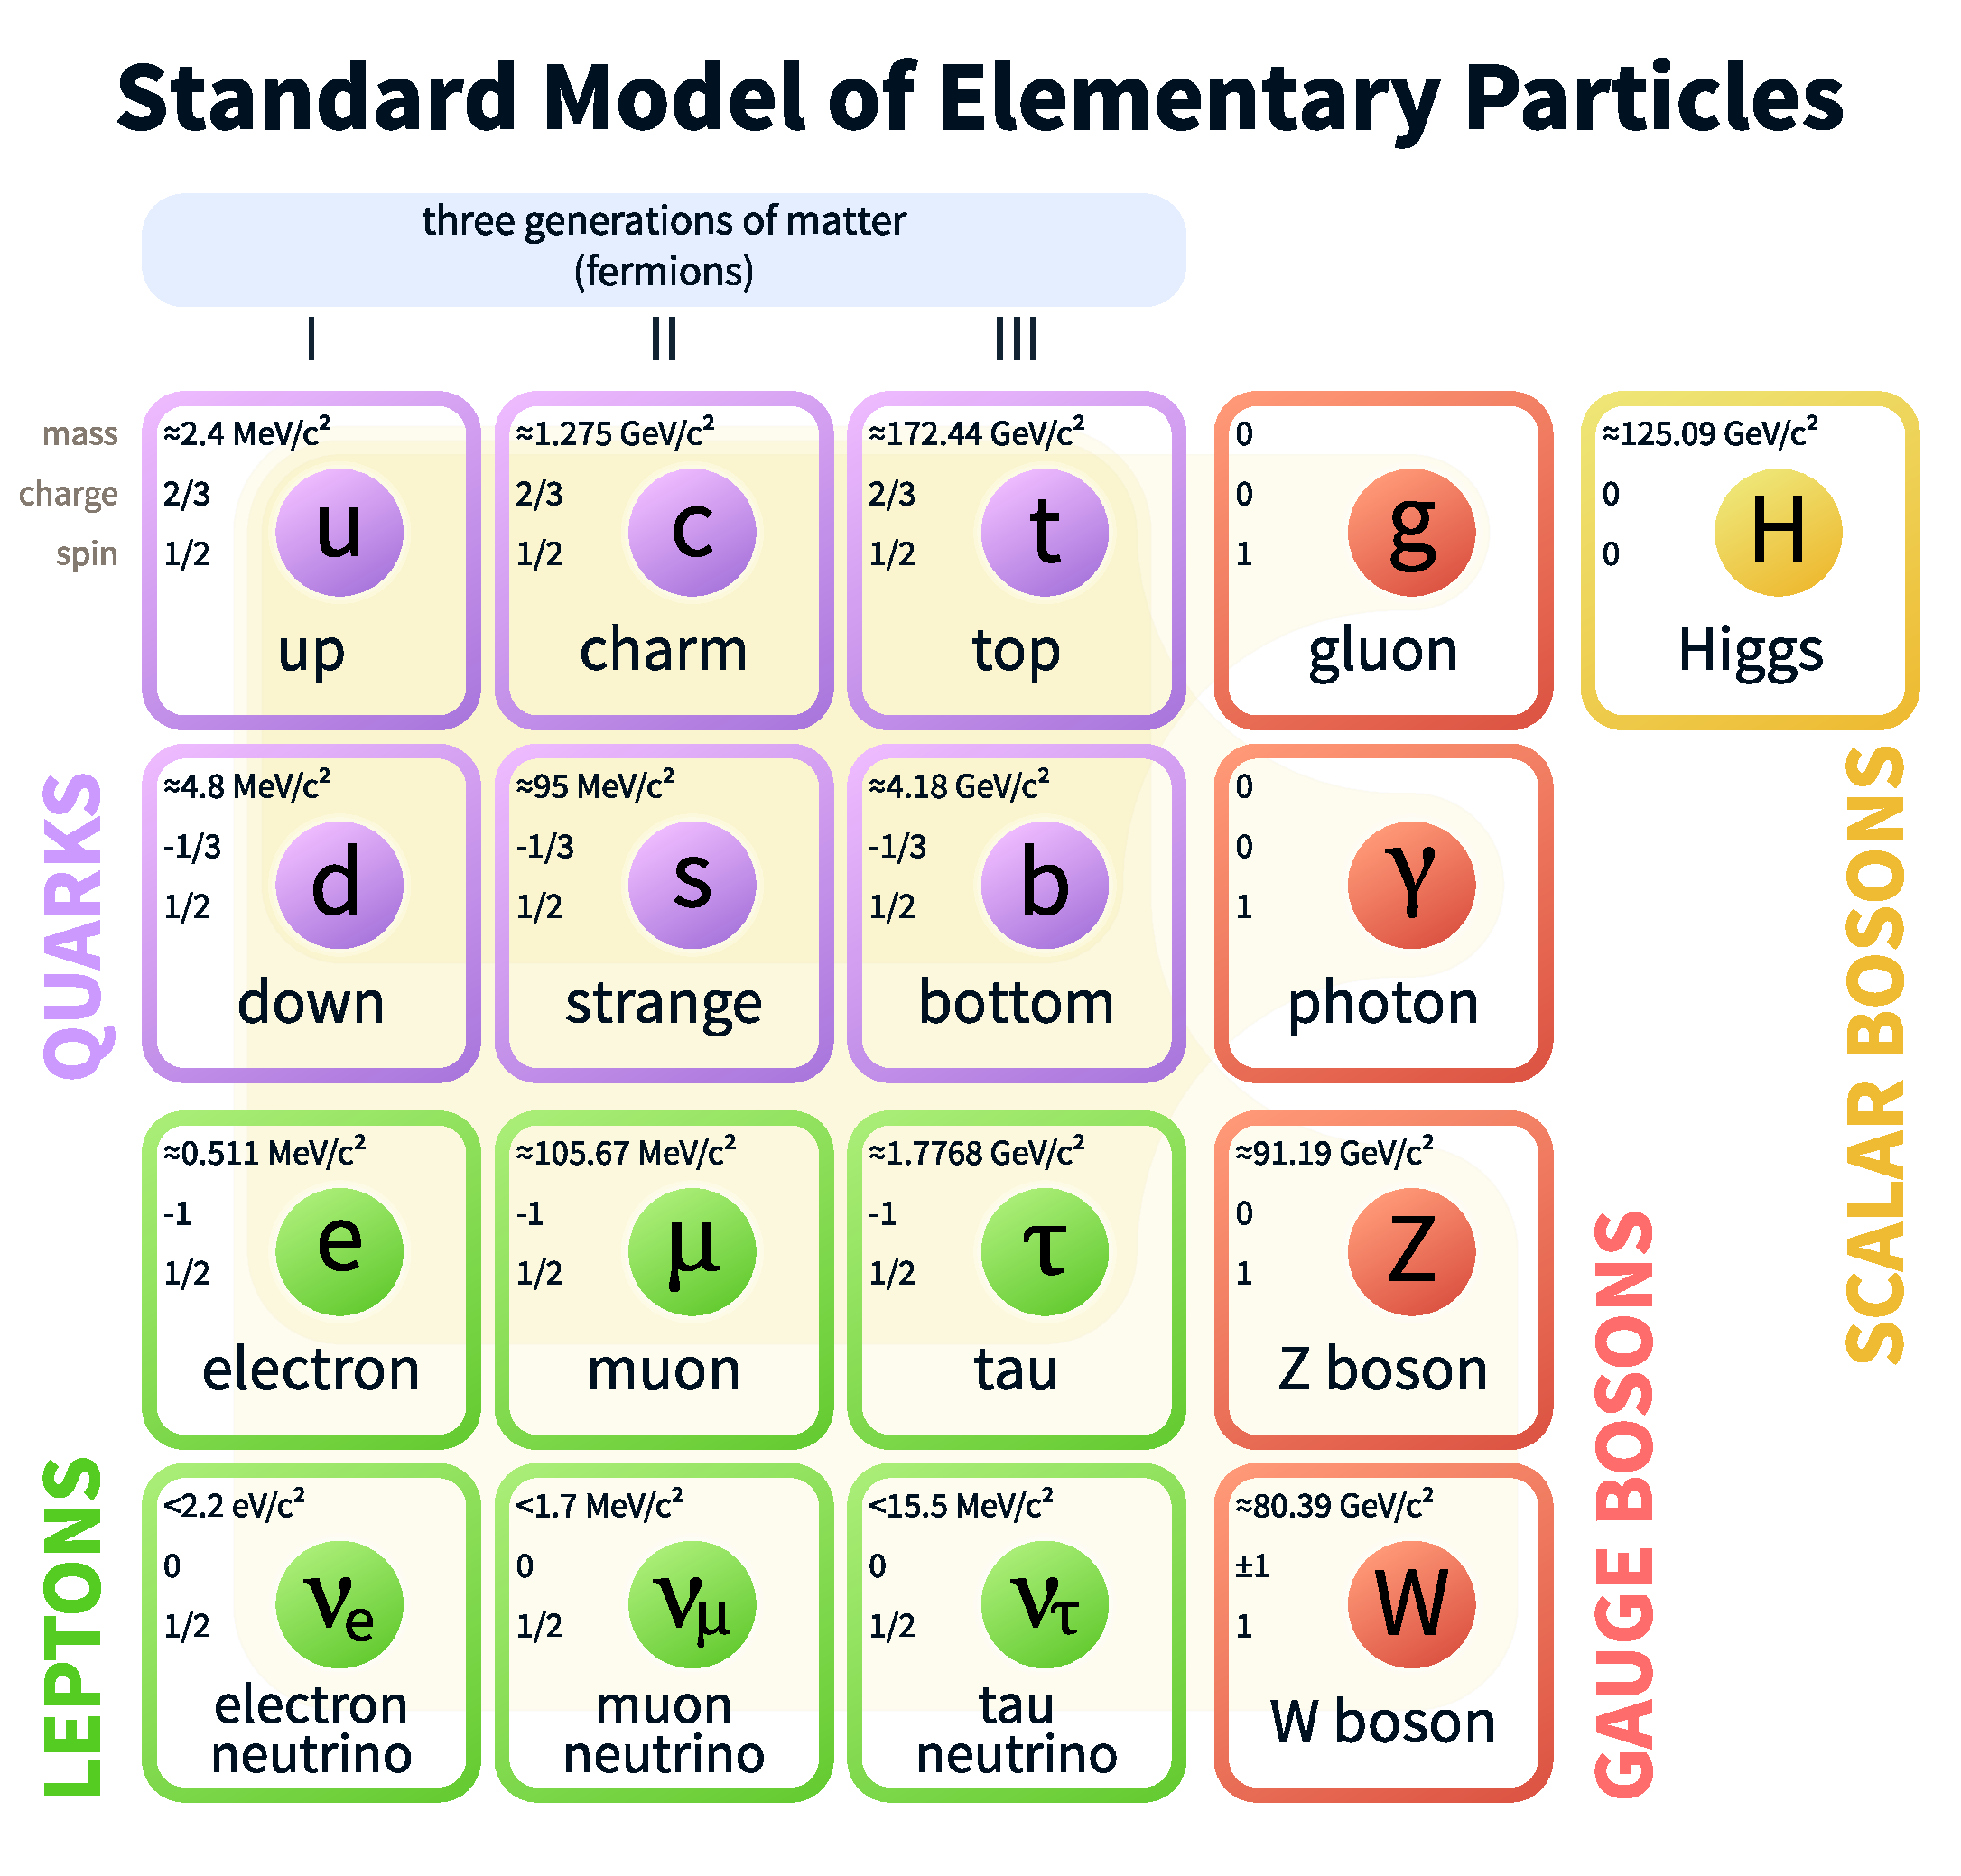
\includegraphics[width=0.9\textwidth]{intro/figs/Standard_Model_of_Elementary_Particles}
	\renewcommand{\baselinestretch}{1.0}
	\caption[An illustration of the elementary particles in the Standard Model and their properties.]{An illustration of the elementary particles in the Standard Model and their properties. The three left columns represent the different generations of fermions, with quarks in purple and leptons in green. The gauge bosons are represented in the fourth column in red, and the only scalar boson, the Higgs, in the fifth column in yellow. \cite{cc}}
	\label{fig:sm}
\end{figure}

\section{Issues with the Standard Model}
\label{sec:smIssues}

Despite the great success of the Standard Model in describing many of the fundamental interactions of particles, it is insufficient to explain all physical phenomena. There are several outstanding theoretical questions left unanswered by the Standard Model, and experimental evidence to suggest it is incomplete.

One of the most perplexing theoretical features of the SM is the fact that we have been able to detect all the elementary particles at energies accessible in our experiments. Because the bare masses of particles in the SM Lagrangian receive corrections from quantum loop diagrams, it is not clear why new particles (which must be massive) do not contribute significantly to these corrections. In particular, the quantum loop corrections to the Higgs boson mass include all massive particles, and contributions from undiscovered massive particles could drive the Higgs mass far beyond what is currently accessible, yet this is not observed. This is often referred to as the {\it hierarchy problem}.

Experimental evidence also suggests there are physical phenomena not explained by the SM. Measurements of the rotational velocity of galaxies compared to the visible matter indicate there is an abundance of {\it dark matter} in the universe which cannot be accounted for by the particle content of the SM \cite{Corbelli:1999af}. Furthermore, while the SM predicts neutrinos to be massless, measurements of neutrino flavor oscillations imply that neutrinos mass is very small, but nonzero \cite{Alberico:2003kd}. Such measured phenomena indicate there may be additional particle content beyond what is posited by the SM, and additional interaction terms between SM particles and a ``dark sector'' of weakly-interacting particles.

\section{Beyond the Standard Model: Supersymmetry}
\label{sec:bsm}

In order to solve many of the theoretical and experimental issues with the SM, theorists had considered extending SM particle content and interactions to include additional species which might satisfy some of the theoretical constraints of the SM in a consistent manner with observation. However, in 1975 the Haag-\L{}opusza\'{n}ski-Sohnius theorem \cite{Haag:1974qh} demonstrated that the only non-trivial extensions of quantum theories do not only include internal symmetries and the Poincar� symmetry, but also a non-trivial extension of the Poincar� algebra known as {\it supersymmetry} \cite{PhysRevD.3.2415, NEVEU197186, Golfand:1971iw, NILLES19841, FAYET1975104, WESS197439, WESS197452, Volkov:1972jx}.

A quantum field theory of supersymmetry (SUSY) can be visualized as a dual version of a typical field theory. For each particle, there exists a superpartner with different spin; fermions have boson-like superpartners and bosons have fermion-like superpartners. This is a particularly appealing and elegant solution to many of the issues with the SM; loop diagram corrections to particle mass are partially cancelled out by contributions from superpartner loop diagrams, providing a natural solution to the hierarchy problem \cite{Martin:1997ns}. In typical ``R-parity conserving'' SUSY theories, particle interactions also conserve ``SUSY-ness'' in decays, and thus when a superparticle decays into SM particles, the cascade will always end in the lightest supersymmetric particle (LSP). The LSP must be stable, and because it interacts very weakly with the SM sector provides a suitable dark matter candidate.

While there are many beyond-SM (BSM) theories that seek to explain phenomena beyond the scope of the SM, SUSY provides both elegant solutions to the theoretical concerns of the SM as well as a robust framework to unexplained physical phenomena. The analysis described here is designed to be model independent in a search for new physics, but also sets constraints on SUSY models as it is one of the more promising BSM theories that might be realized by nature.
% --------------------------------------------------------------------------- %
% --------------------------------------------------------------------------- %


%% \bibliographystyle{lucas.bst}
\bibliographystyle{plain.bst}
%% \justify
%\bibliography{include/refs}

\appendix

\end{document}
